\chapter{Current APIs\label{section:currentAPIs}}
\textbf{TODO: write each introduction chapter in the same style, currently
each slightly differ}

In this chapter we will first give an overview of what APIs are available for
use, after which we will compare the APIs with features, finally covering
feature differences and performance statistics. Unfortunately there are no
direct statistics that show how much each API is used. Some were gathered
through interviews, although the sample size is not large enough to say
conclusively whether one is used more or another.

\section{Introduction to camera APIs}
\subsection{Video For Linux 2}\label{section:v4l2}
\textit{Video For Linux 2} (V4L2) serves as the fundamental low-level API
within Linux\footnote{https://www.kernel.org/doc/html/v4.9/media/intro.html}.
It's designed for managing video capture and output devices (among other things
like radio). It serves as the foundation for many of the higher-level APIs that
offer more user friendly approaches for video processing. V4L2 uses a very
minimalist approach, providing the user with great control over the camera
devices, with standard ways to control almost any camera device.

V4L2 is a very low level API, it does not provide any of the convenience
features found  in modern APIs. This allows V4L2 to have a very intricate
control over the camera, though requiring more management by the developer.
Being a C api, there are few encapsulating structures for things like images.
Instead everything is treated as buffers that the user must manage directly,
this can lead to more complexity and potential errors as developers are known
to not be very good at this~\cite{van2012memory}. The camera is controlled
using \textit{ioctl} commands. \textit{ioctl} commands are ways to configure
devices that normally are not configurable by file operations directly.

V4L2 still is widely used in fields such as robotics\footnote{Personal
communication, October 2024}, although hopefully we will move away from it once
libraries like Argus and libcamera gain traction.

V4L2 is split into two libraries, the kernel side which is known as V4L2, and the
userspace library known as libv4l2. The userspace library often just wraps the
kernel functions and forwards the arguments to the kernel API.

\subsection{Argus}
%https://docs.nvidia.com/jetson/l4t-multimedia/group__LibargusAPI.html

Argus is a camera API that is developed by Nvidia. Argus runs only on Nvidia
hardware, such as the Jetson Orin Nano Developer Kit.

Argus is roughly based on V4L2 though effectively a re-implementation. At the
time Argus was created, V4L2 was still in an early stage. It di not supporting
a variety of features such as multicamera setups etc. hence Argus was created
in order to add the missing features easily. These days V4L2 and Argus are very
close though in later chapters we will give an overview of what pros and cons
each has.

The reason Argus does not use V4L2 is largely a historical one at this point.
At the time Argus was created V4L2 was in an early stage, it had very limited
features. Nvidia created Argus in order to leviate these issues but ended up
with an API that is very similar to V4L2. Automotive for example needed support
for multi camera use cases, this was something that was not supported in V4L2 at
the time.

Over time, the API has aged a little though. Today it is still very dependent
on EGL. Like OpenGL, EGL is a very old API, today it does not receive much
updates. Effectively only when requested by big customers, even then it is
almost exclusively to enable emulation using Vulkan\footnote{Tony Zlatinski,
Personal communication, October 2024}. The issue with OpenGL and EGL is that it
assumes an internal state. While this state allows users to create applications
quickly, avoiding much boilerplate, it also sets a "glass ceiling". This
ceiling sets a limit on how fast applications can run as certain things can not
be optimized.

There is an additional camera API from Nvidia that we will not cover, namely
SIPL. This requires Nvidia specific hardware that is not easy to acquire. The
main difference with it is that it's a streaming based API that is safety
certified\footnote{\href{https://developer.nvidia.com/docs/drive/drive-os/6.0.8.1/public/drive-os-linux-sdk/common/topics/nvmedia\_concept\_nvsipl/PlatformCameraConfiguration.html}{developer.nvidia.com}},
meaning it can be used in automotive.

\subsection{libcamera}
\begin{figure}
    \begin{center}
        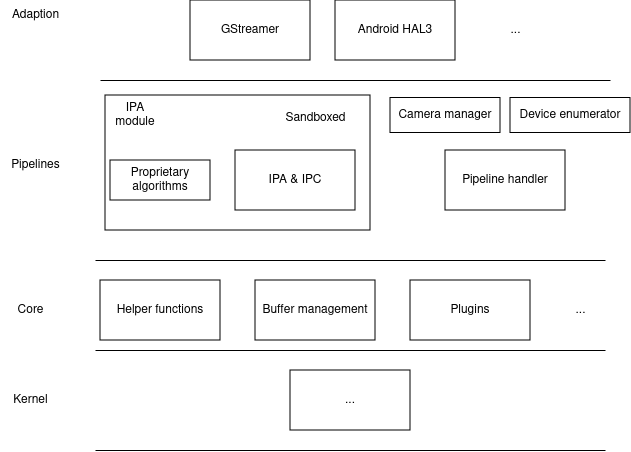
\includegraphics[width=0.60\textwidth]{figures/libcameraarch.png}
    \end{center}
    \caption{High level overview of how the libcamera architecture looks like}
    \label{fig:libcameraarch}
\end{figure}

libcamera is an open-source C++ embedded camera framework that supports a large
number of complex cameras. Complex cameras are cameras that require heavy
hardware image processing, such as the Sony IMX 219, 477 and many more. It
supports multiple encoders to receive images in for example PNGs/raw images.
The primary target for libcamera is ARM processors in the form of Raspberry
PIs, Chromebooks and Android mobile phones though many other architectures are
also supported~\cite{libcameraStack}. Because image processing algorithms are
often proprietary and very secret, libcamera also allows for binary blobs to be
supplied by the vendors. The vendors do need to submit the "base case" where
the camera can take a still image with decent quality to get the blob approved.
These blobs are run in a separate process, communicating with libcamera though
an API provided by the Pipeline Handler using \textit{dmabuf} handles. These
\textit{dmabuf} handles are very effective due to the fact that they do not
require copies. If the user wants to read the buffer, it can be mapped using
\textit{mmap}. By default this is not done, as mapping it would require the
\textit{Memory Management Unit} (MMU) to actually copy the data which requires
work.

In \cref{fig:libcameraarch} we can see an overview of how libcamera looks like
from a birds eye view. libcamera provides buffer management along with a lot of
helper functions that allow the vendors to focus on what really matter; the
IPAs. The vendors are encouraged to open source the IPAs as maintaining a fork
is expensive. Additionally if the IPA is closed source there are some
restrictions: in order to ensure that the IPAs do not run any malicious code it
has a very limited access to the kernel, no network access, and a very
restricted view of the filesystem. Open source IPAs do not have these
restrictions, being verified by the maintainers that they do not have any
malicious code. Though as mentioned in the \cref{section:history} chapter,
there are "smart sensors" where the sensor itself has an integrated ISP. These
do not require IPAs and can instead be used as is. IPAs are only required when
the ISP is controlled by the CPU\cite{libcameraStack}.

libcamera then provides high level interfaces then that for example
\textit{GStreamer} etc. can use. This allows each application to simply build on top
of the same API for each ISP.
\textbf{TODO: describe capture process like in HAL3}

\subsection{HAL3}
Hardware Abstraction Layer 3 (HAL3) is the camera API that is included in each
Android phone, it has remarkable features for a mobile phone camera. It was
created to bridge the gap between the higher level API camera2\footnote{https://source.android.com/docs/core/camera/camera3}
and the lower level hardware APIs. It allows for more modification than
camera2, while requiring more work to manage.

Like libcamera and Argus, it is a request based API. Being a request based API
allows it to be a very explicit API and allows for the user to have a
significantly higher level of control. The reason for the other two being very
close to HAL3 in style is because they are largely based on it, and Frankencam.
Both Argus and libcamera provide HAL3 support.

While request based APIs allow for a better control of the camera, it also
makes it so that the API is not able to optimze much if the request can fully
change each frame. While if the API was a streaming API it could have certain
assumptions that reduce amount of copies. Hence making it faster.

In \cref{fig:hal3arch} we can see the high level diagram of how a capture
request is done and how the frame arrives to the end user. The capture process
works in the following way:

\textbf{TODO: describe opening and closing the camera and how it ties into libcamera}
\begin{enumerate}
    \item Create a capture request, modifying gain, focal length etc.
    \item Give capture request to the capture device class
    \item Capture device passes the request to the ISP which creates a program
        for the request, see \cref{section:isp} for a detailed explanation of
        how ISPs work.

    \item Images come in the form of a capture result to the application.
\end{enumerate}


\begin{figure}
    \begin{center}
        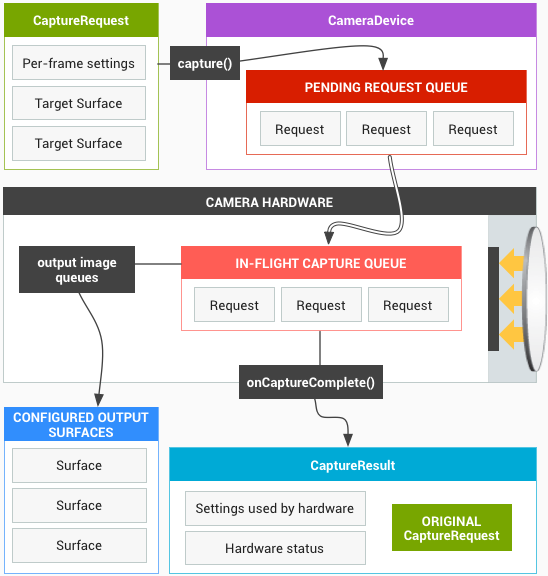
\includegraphics[width=0.5\textwidth]{figures/hal3arch}
    \end{center}
    \caption{HAL3 architecture~\cite{hal3arch}}\label{fig:hal3arch}
\end{figure}

\subsection{Kamaros}
Over the years there have been some camera standardization efforts such as
OpenKCam. These have failed though due to lack of industry interest. Today
the Khronos group has started the camera standardization effort again with
Kamaros.

Kamaros is a new API currently (2024) being designed. Its goal is to
standardize embedded camera frameworks. This means that instead of needing
three different APIs for Android, L4T, and Linux you would only need to use
Kamaros. It would sit on top of the transport layer (CSI-2, USB etc.), allowing
the applications to use a single API to communicate with cameras over multiple
platforms. Though there are still many other issues in the camera world that will not
be solved by Kamaros. Examples of these are for example camera configuration.
Currently there is no standard way to configure cameras, the camera drivers are
often a huge part of the code base. At the same time, there is not a lot of
difference between them. In the future, Kamaros may try to tackle this problem
though it is not anything that will be solved initially.

The API is under development, so not much can be mentioned about the API itself
due to a spec not being out yet. It hopes to be easy to use and ability to
leverage Vulkan for post processing. This would allow users to easily create
cross platform code and not be highly platform dependent as it is currently.
\cref{fig:kamaros_stack} shows where it would fit in a typical application.

\begin{figure}
    \begin{center}
        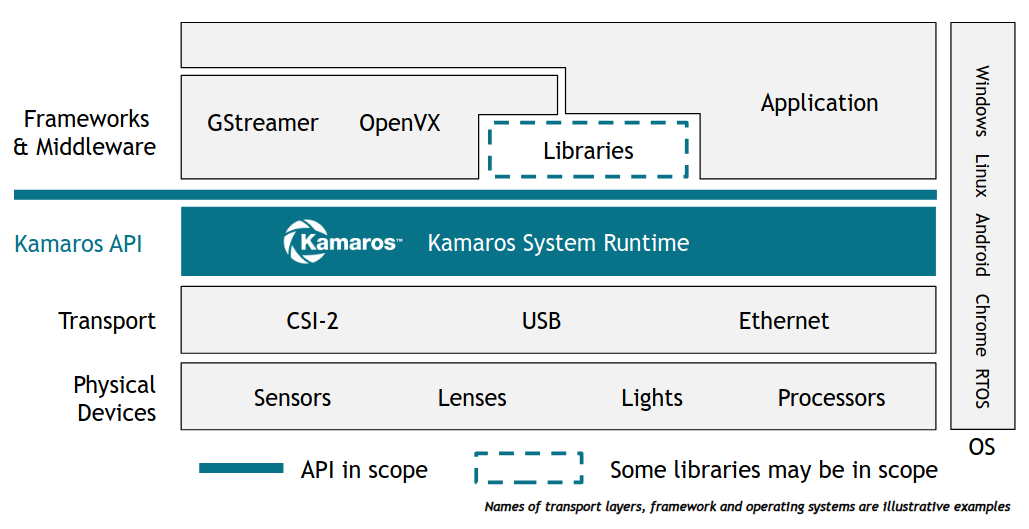
\includegraphics[width=0.60\textwidth]{figures/kamaros_stack.png}
    \end{center}
    \caption[Kamaros stack]{Kamaros stack, \textit{image source: \href{https://www.khronos.org/assets/uploads/developers/presentations/Khronos\_Kamaros\_Embedded\_World\_Mar23.pdf}{Embedded world}}}\label{fig:kamaros_stack}
\end{figure}
\footnotetext{}

\subsection {GenICam}
\textit{Generic Interface for Cameras} (GenICam) is a standard\footnote{\href{https://www.emva.org/wp-content/uploads/GenICam_Standard_v2_1_1.pdf}{GenICam Standard.pdf}} that was
developed by the \textit{European Machine Vision Association} (EMVA). It is
largely used by industry.

Genicam is a significantly higher level API than the ones listed above. It
uses for example XML files to configure cameras, this is not very space
efficient compared to device trees. Genicam libraries are often provided by the
sensor manufacturer. Like other APIs though, it deals with the same problem:
configuring cameras.

\section{API Comparison}\label{section:comparison}
While the APIs largely do the same thing, in a very similar fashion they still
have different use cases. Each still provide unique features when it comes to
both camera control, image processing, and the platforms they run on.

libcamera runs on essentially any platform that can run linux, except for
tegra devices running \textit{Linux For Tegra} (L4T). libcamera does not run
on L4T because the L4T V4L2 implementation has strayed too far from the
upstream version\footnote{https://github.com/kbingham/libcamera/issues/81}.
While Argus only runs on Android and L4T. Finally, HAL3 runs on any platform
that can run Android.

When familiarizing oneself with the different APIs, currently Argus is the most
difficult to learn. There are multiple samples that can be looked
at though all of them are quite advanced. These examples do not
have many comments and do not cover the "base case" of capturing an image. They
do not have many comments either, requiring you to decipher what the code does.
Additionally these examples require you to buy a Jetson (Orin) Nano in order to
view them as they're not hosted online anywhere. libcamera on the other hand
provides a very good simple example of how to use the API\footnote{\href{https://github.com/kbingham/simple-cam/blob/master/simple-cam.cpp}{simple-cam.cpp}}.
It has an explanation on everything it does almost line by line, providing
ASCII images explaining for example hardware blocks.

CUDA is a very popular way to program GPUs~\cite{kalaiselvi2017survey}, this
puts gives Argus a unique standing where it supports CUDA very well. libcamera
on CUDA does not support importing DMA buffers very well, this is because DMA
symbols are not exported to non GPL drivers\footnote{\href{https://github.com/torvalds/linux/blob/master/drivers/dma-buf/dma-buf.c}{dma-buf.c}}.
This means that Nvidia drivers aren't able to properly utilize the feature,
which in turn also has a negative side effect where libcamera gives DMA buffers
to the user, CUDA can't import them. There was an effort in 2012 to make DMA
symbols exported to non-GPL code\footnote{\href{https://patchwork.kernel.org/project/dri-devel/patch/1349884592-32485-1-git-send-email-rmorell@nvidia.com/}{Mailing list}}
though it did not get approved.
